\documentclass[a4paper,12pt]{article}
\usepackage{a4wide}
\usepackage{acronym}
\usepackage{graphicx}
\usepackage[title,titletoc,toc]{appendix}


\begin{document}

\begin{center}
{\LARGE\bf Travelling Thief Problem (Multi-Objective)}\\
\vspace{0.5cm}
{\Large\bf Evolutionary Computation}\\
\vspace{1cm}
Prepared by William Reid, Matthew Hart, Samantha Peachey \& Alec Bellati\\
\vspace{1cm}
School of Computer Science,\\
The University of Adelaide\\
\vspace{1cm}
\today
\end{center}


\section*{Exercise 1}

For this section of the assignment, we were required to visualise the datasets ZDT2 and ZDT3 for population sizes 10, 100 and 1000. These visualisations can be found below, with the ZDT2 dataset on the left in blue, and the ZDT3 dataset on the right in red.  Unfortunately, neither dataset provides any insight into what the functions are, and only describe them as Function G and Function H. This makes it hard to comment on the accuracy of these results, however as the population size increases, the shape of the results becomes more defined. With a population size of 10, the ZDT2 graph appears to be a downwards curve, which is reflected in the larger graph sizes. However, the ZDT3 graph on a population size of 10 provides no real insight into the trend of the results, but as the population size increases, the trend becomes much clearer. It is possible to compare the ZDT3 population size 10 graph to the larger population sized graphs and see that it does indeed follow the same trend. 

\begin{figure}[h]
\centering
\begin{minipage}{.5\textwidth}
  \centering
  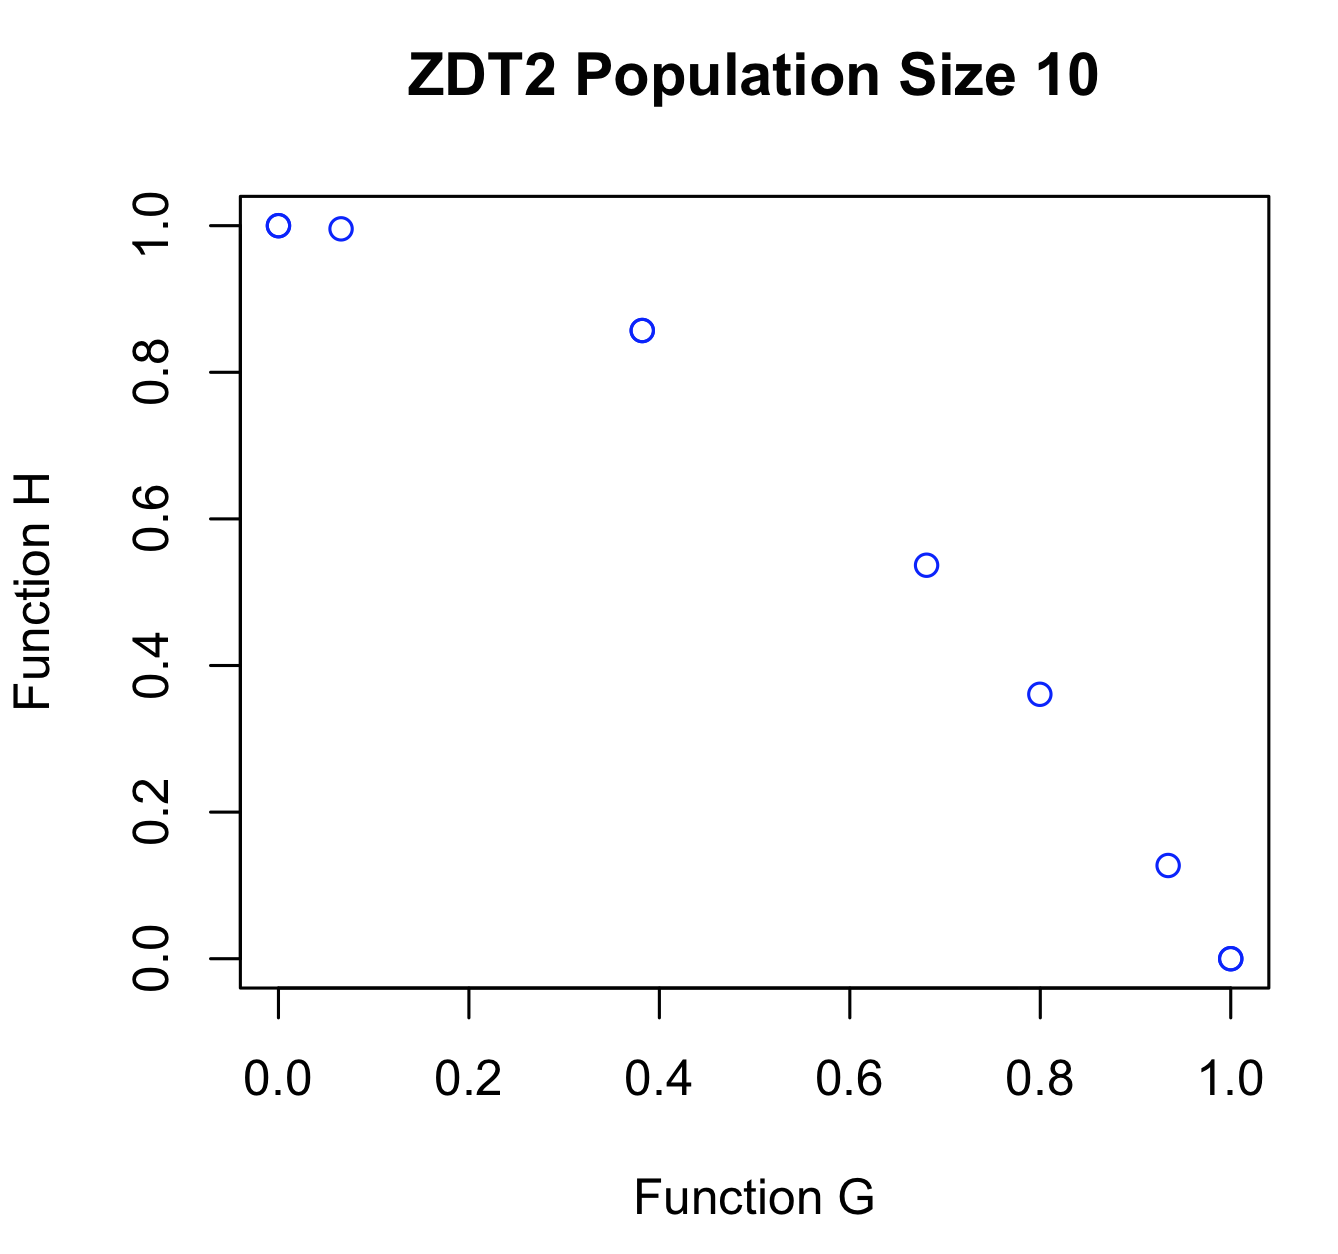
\includegraphics[width=.8\linewidth]{q1graphs/zdt2_10.png}
  \label{fig:zdt210}
\end{minipage}%
\begin{minipage}{.5\textwidth}
  \centering
  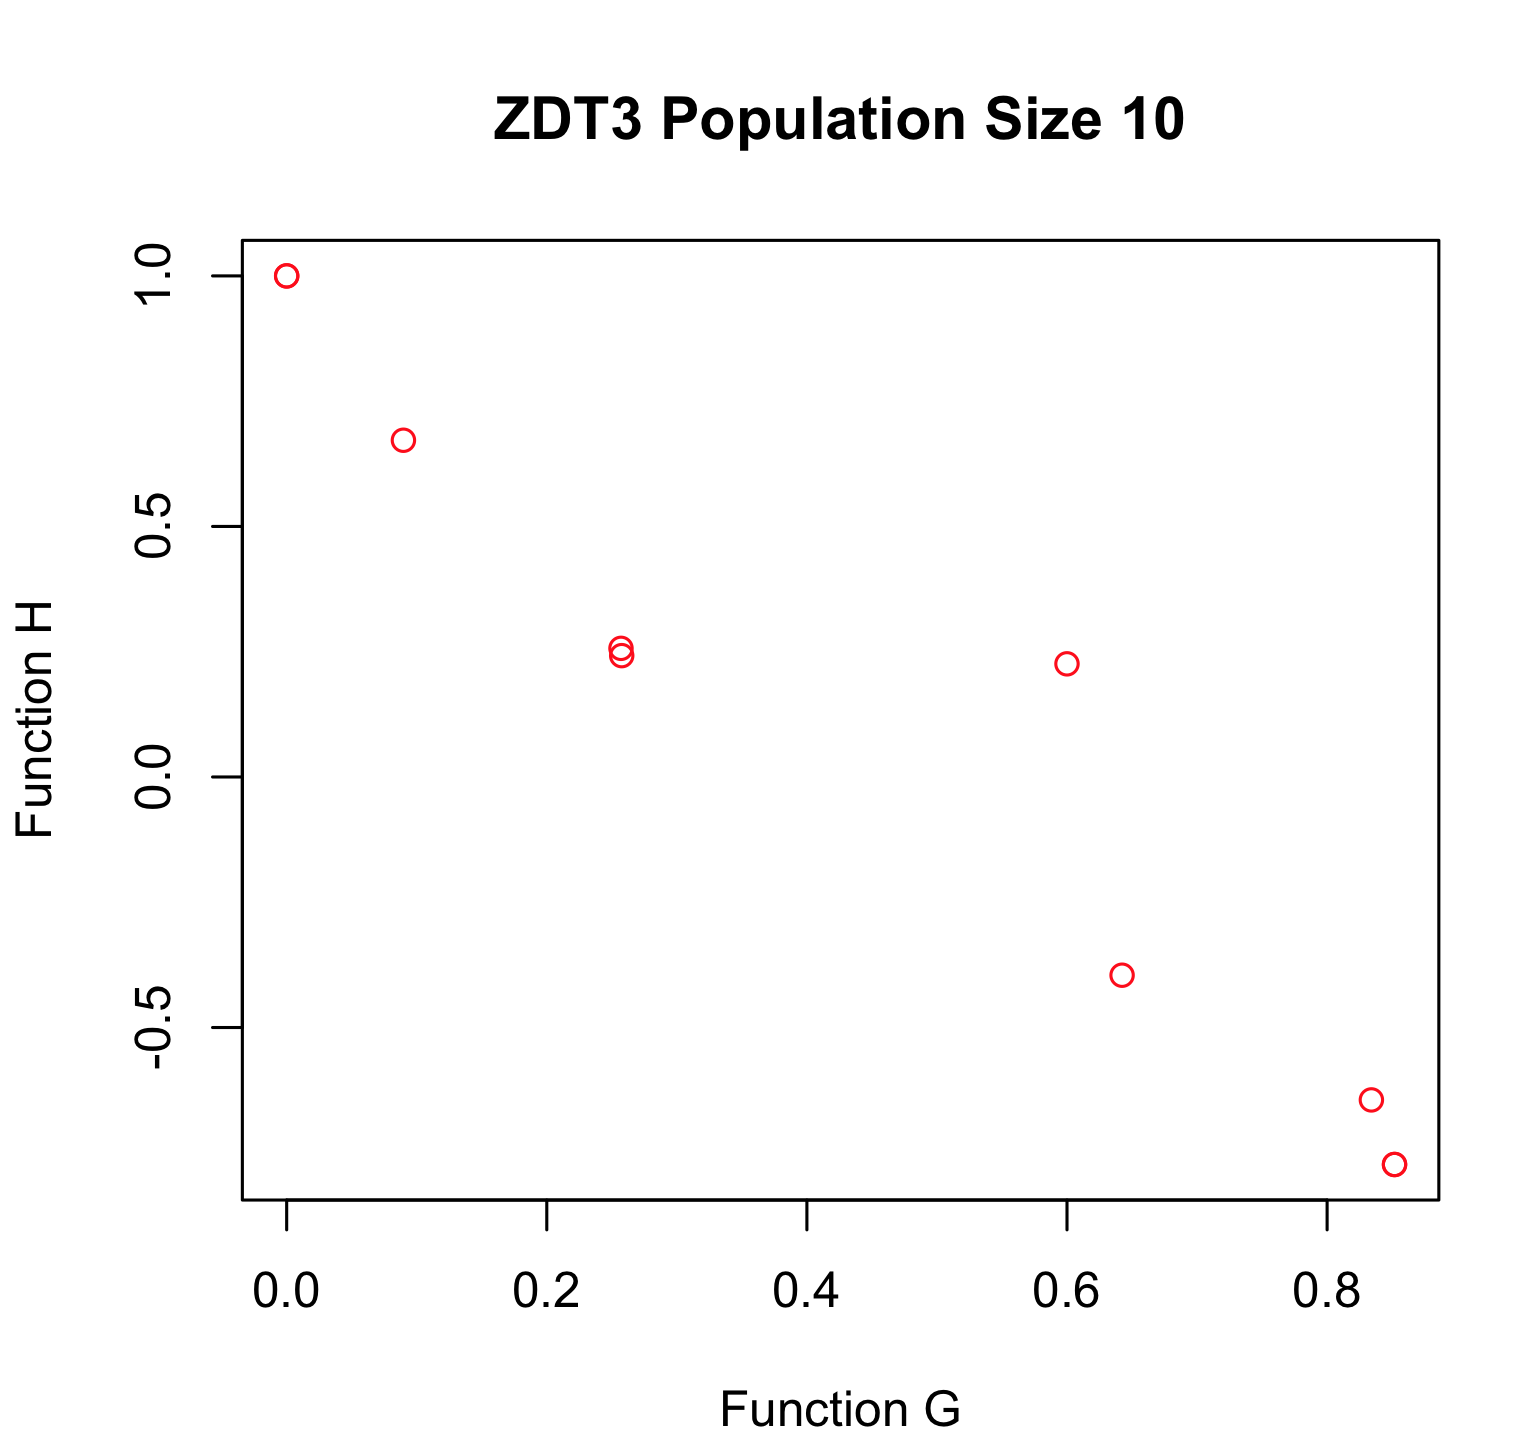
\includegraphics[width=.8\linewidth]{q1graphs/zdt3_10.png}
  \label{fig:zdt310}
\end{minipage}
\end{figure}

\begin{figure}[h]
\centering
\begin{minipage}{.5\textwidth}
  \centering
  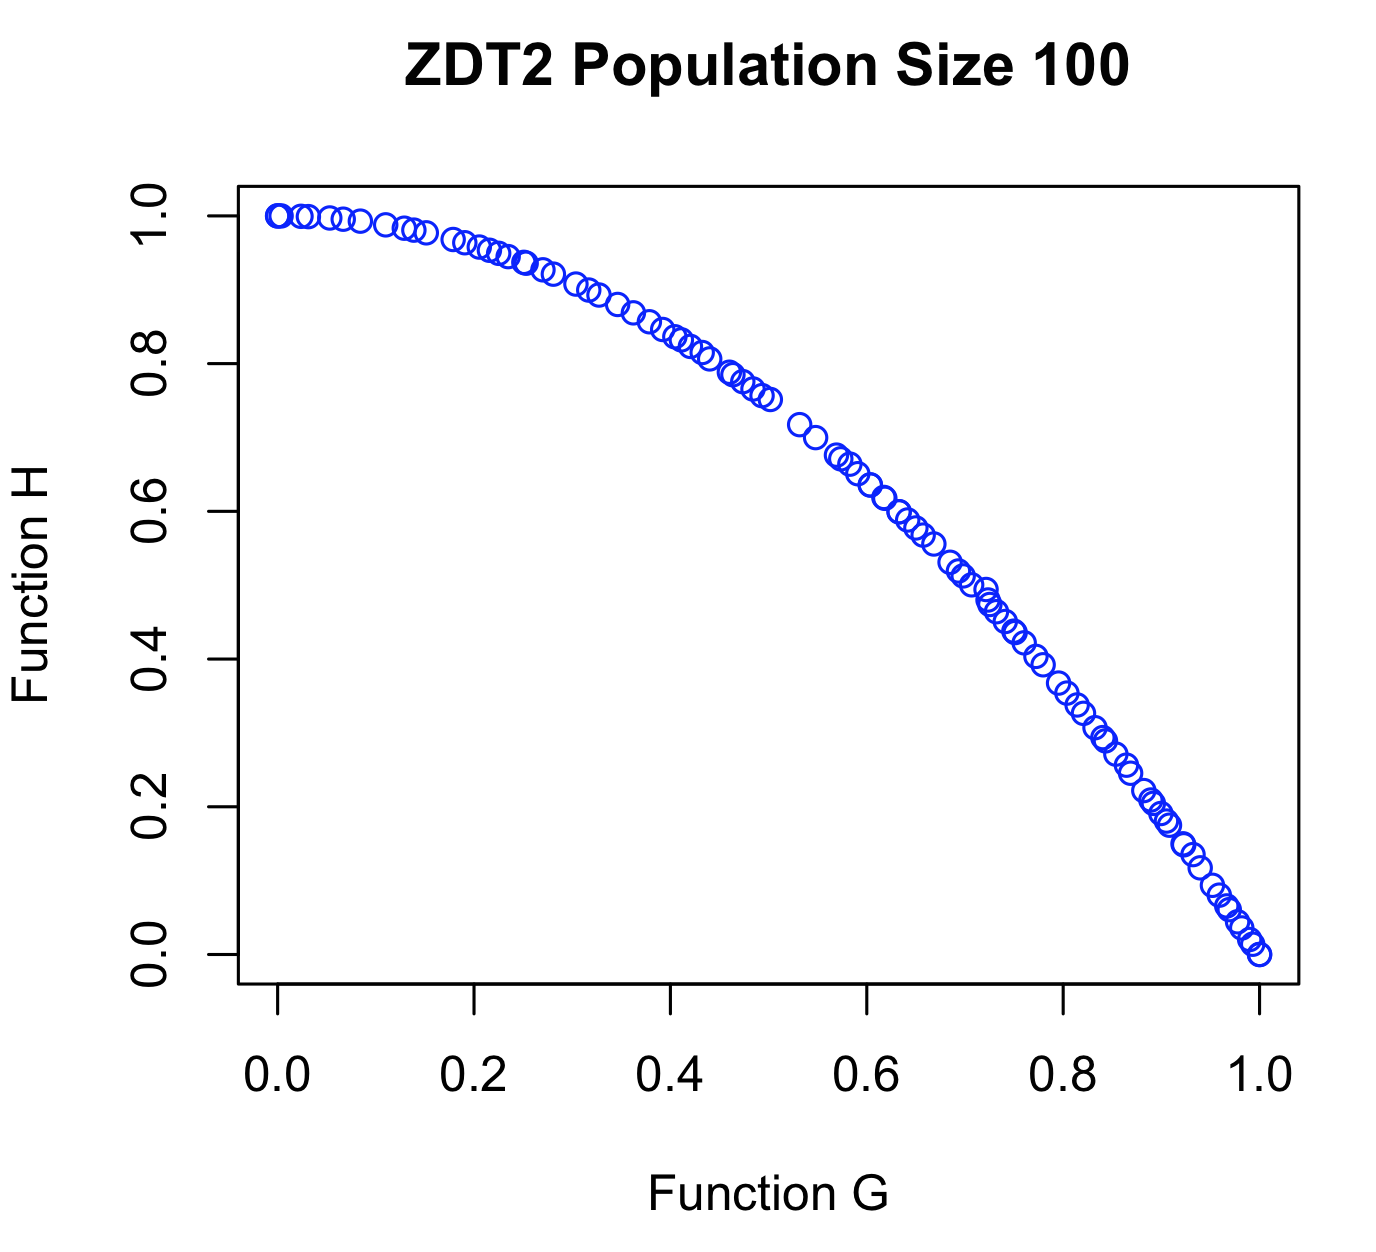
\includegraphics[width=.8\linewidth]{q1graphs/zdt2_100.png}
  \label{fig:zdt2100}
\end{minipage}%
\begin{minipage}{.5\textwidth}
  \centering
  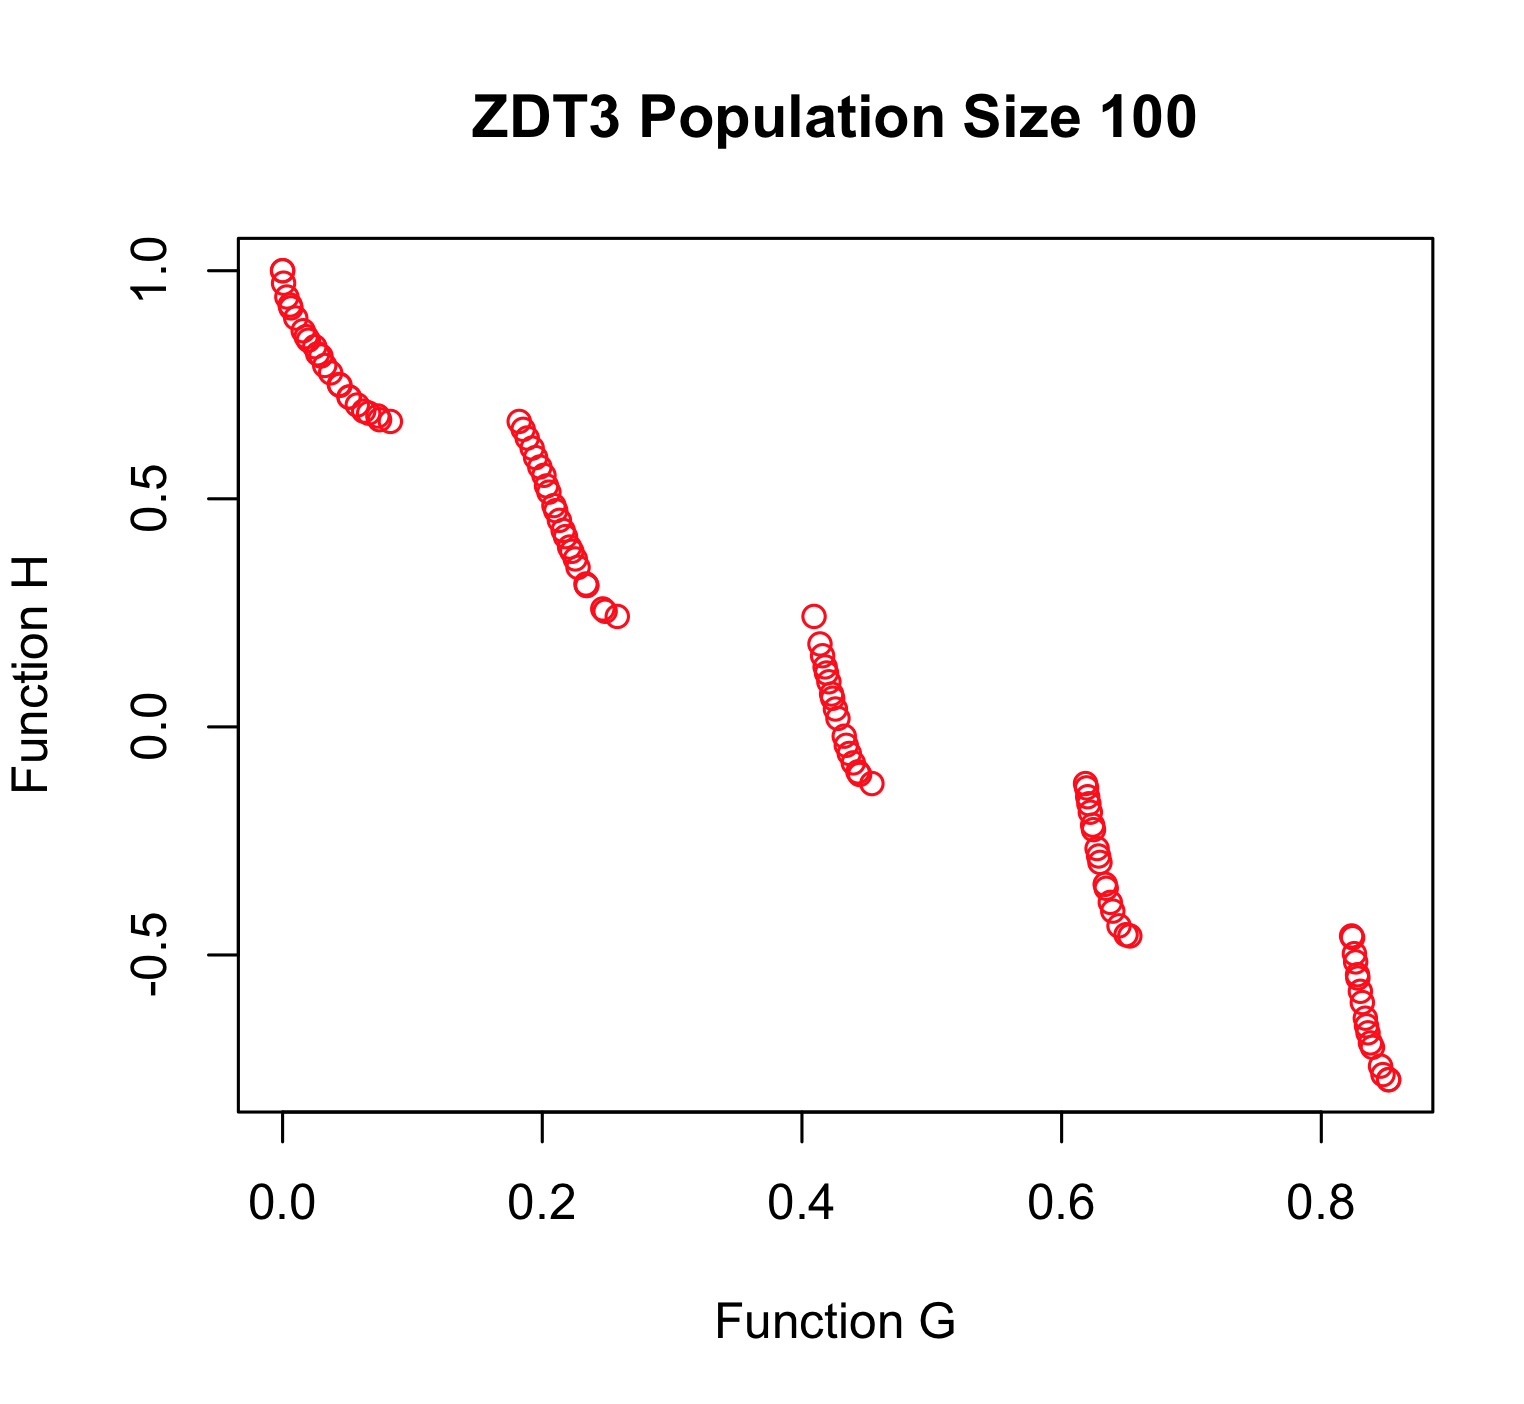
\includegraphics[width=.8\linewidth]{q1graphs/zdt3_100.png}
  \label{fig:zdt3100}
\end{minipage}
\end{figure}

\begin{figure}[h]
\centering
\begin{minipage}{.5\textwidth}
  \centering
  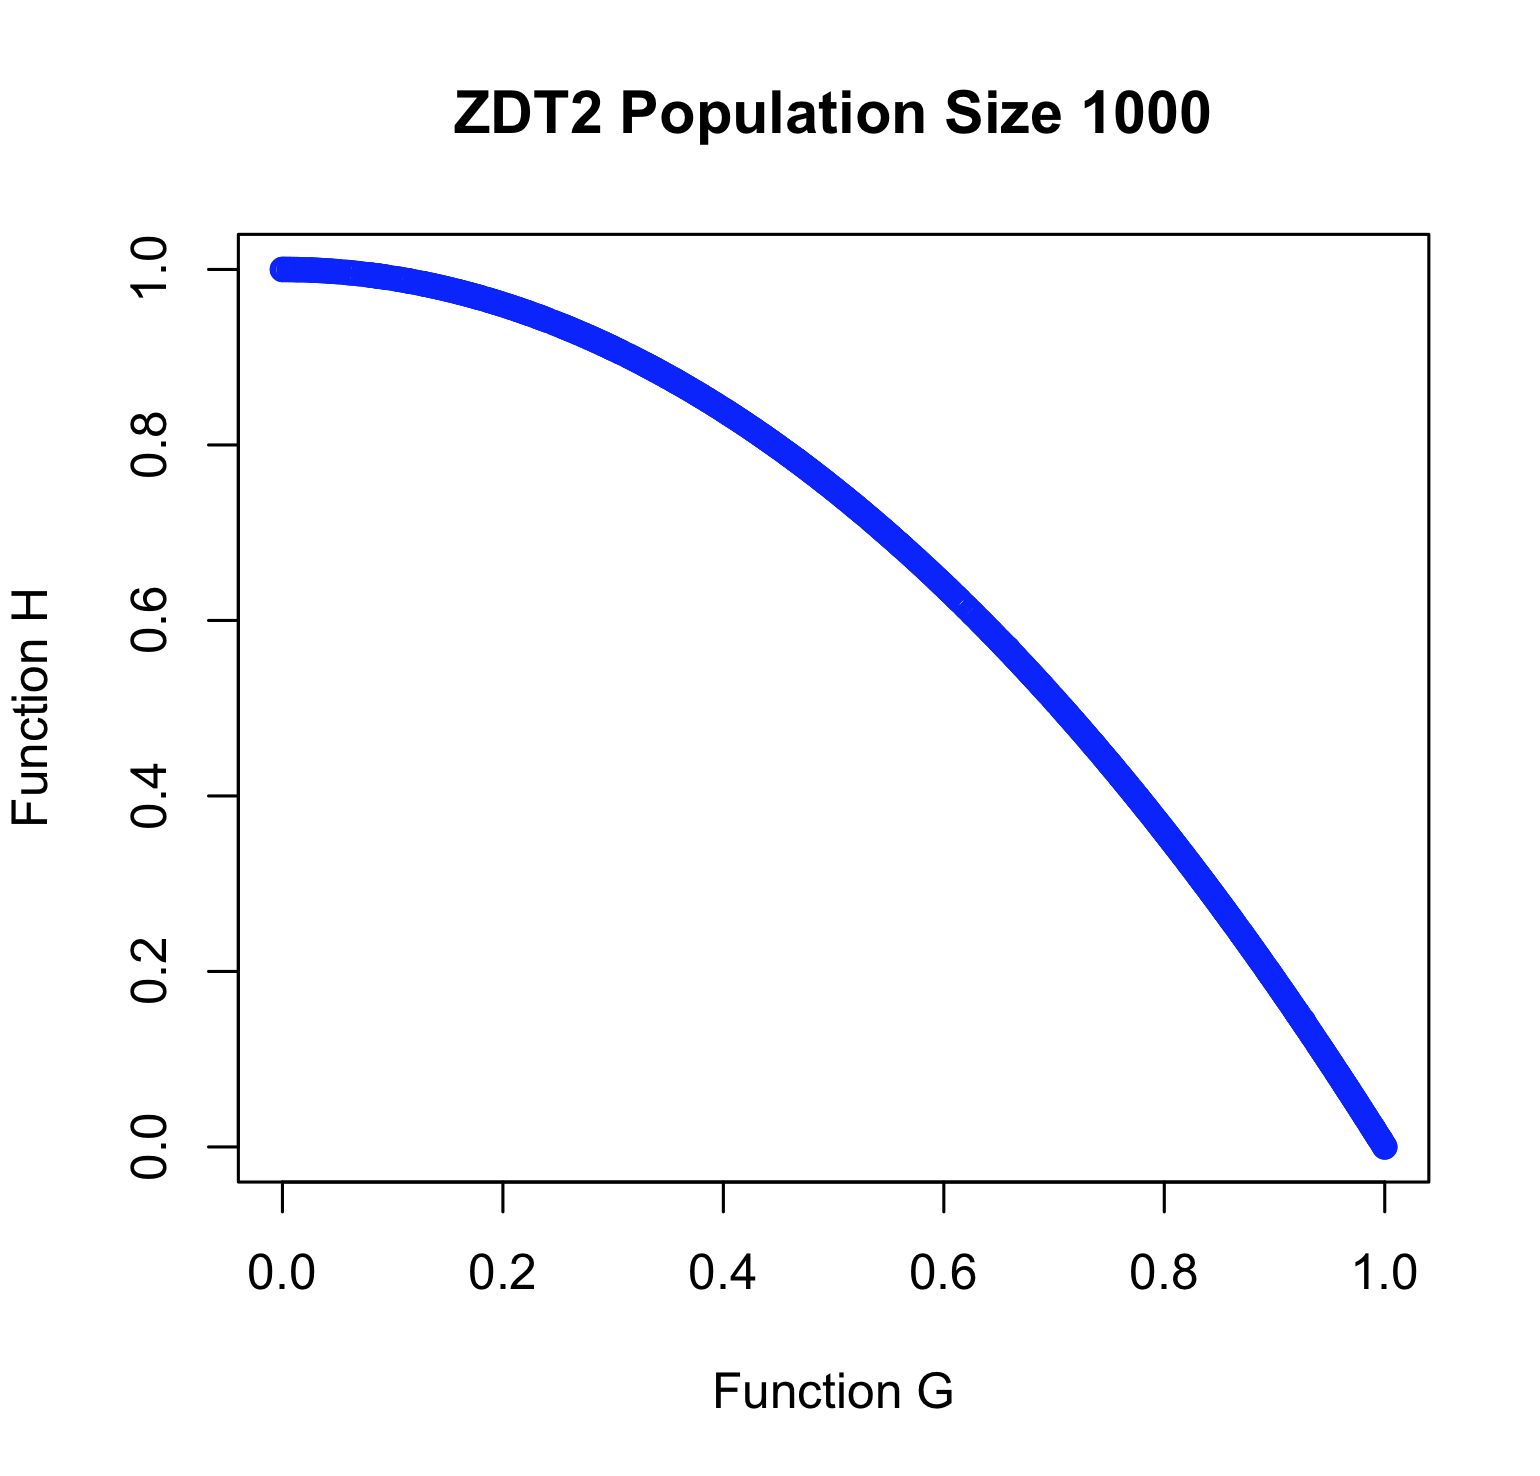
\includegraphics[width=.8\linewidth]{q1graphs/zdt2_1000.png}
  \label{fig:zdt21000}
\end{minipage}%
\begin{minipage}{.5\textwidth}
  \centering
  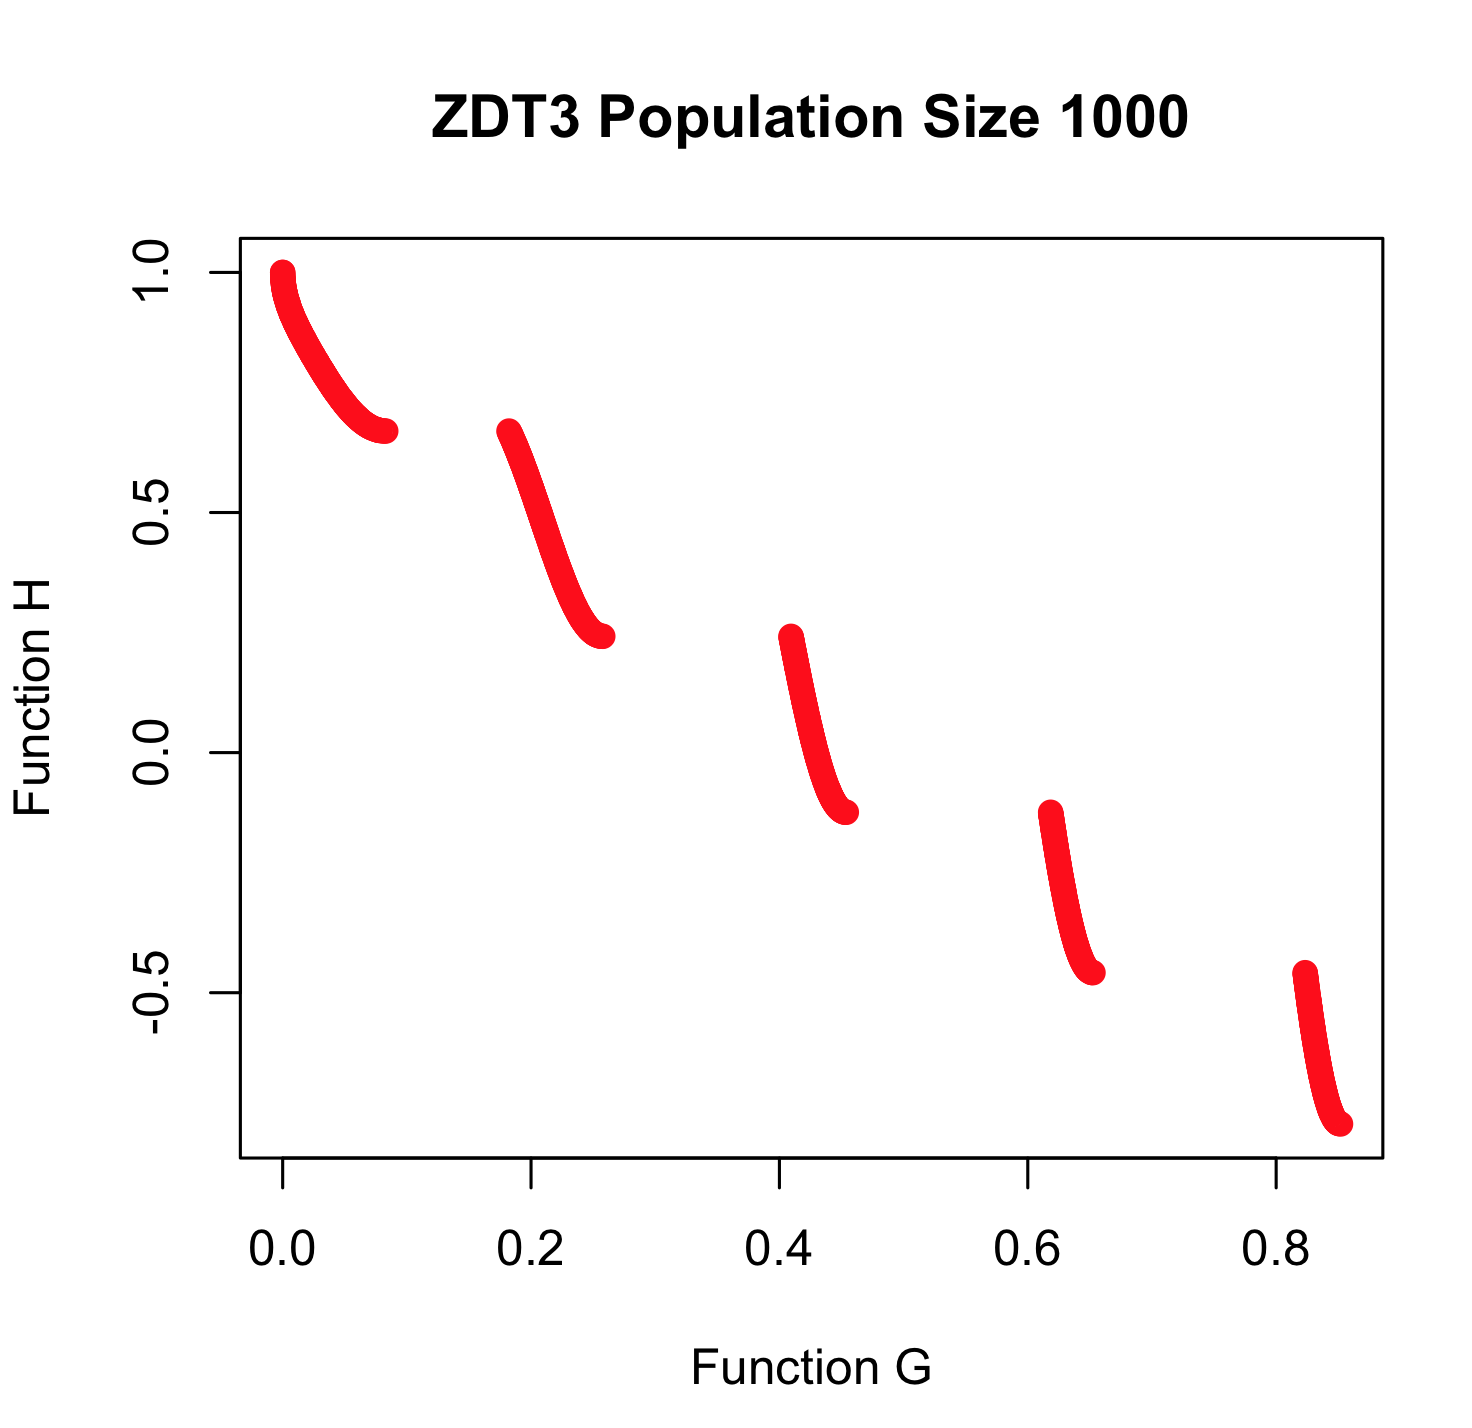
\includegraphics[width=.8\linewidth]{q1graphs/zdt3_1000.png}
  \label{fig:zdt31000}
\end{minipage}
\end{figure}

\section*{Exercise 2}
Discuss where to find these things here

\section*{Exercise 3}
Again discuss where to find these things here

\section*{Exercise 4}
Maybe some discussion on the results here or something idk



\begin{figure}[h]
\centering
\begin{minipage}{.5\textwidth}
  \centering
  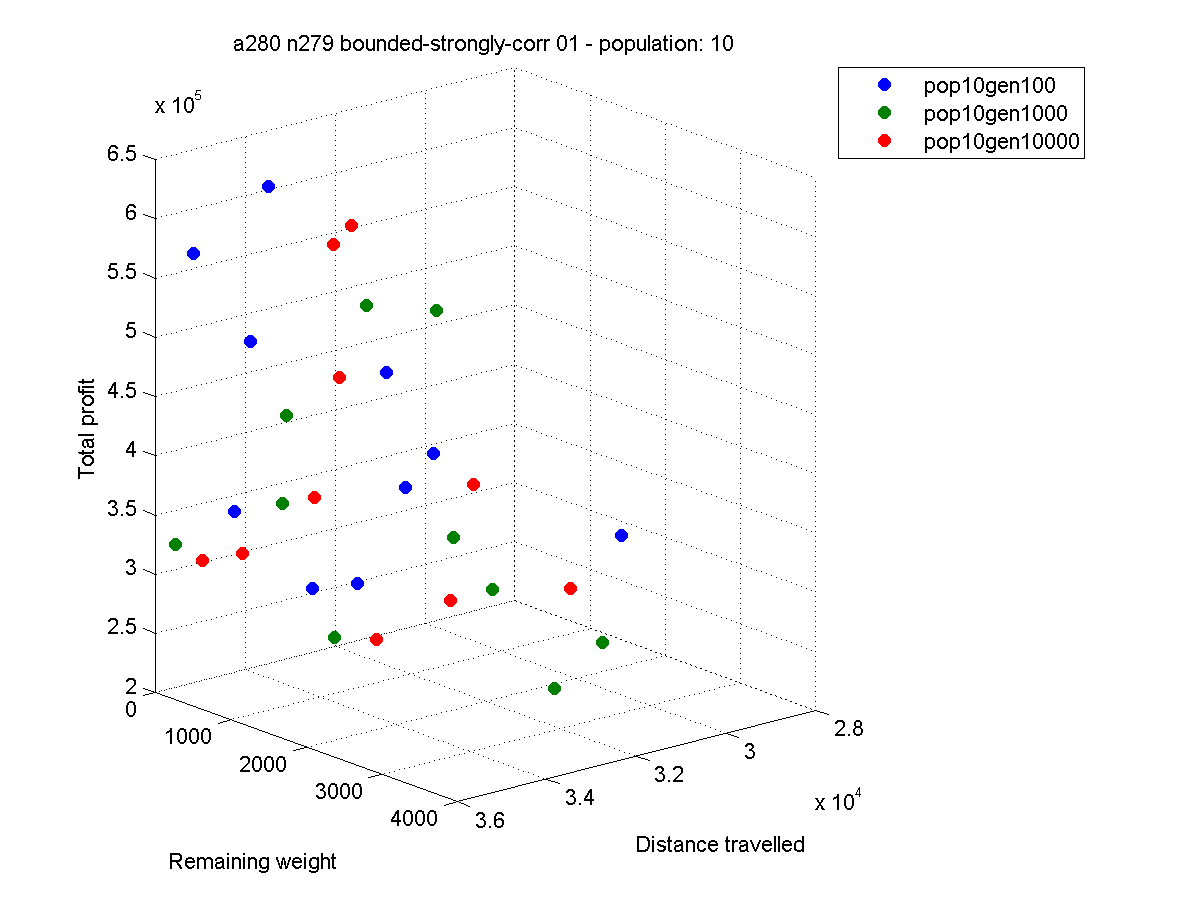
\includegraphics[width=.8\linewidth]{q4graphs/a280_n279_pop10.png}
  \label{fig:a28027910}
\end{minipage}%
\begin{minipage}{.5\textwidth}
  \centering
  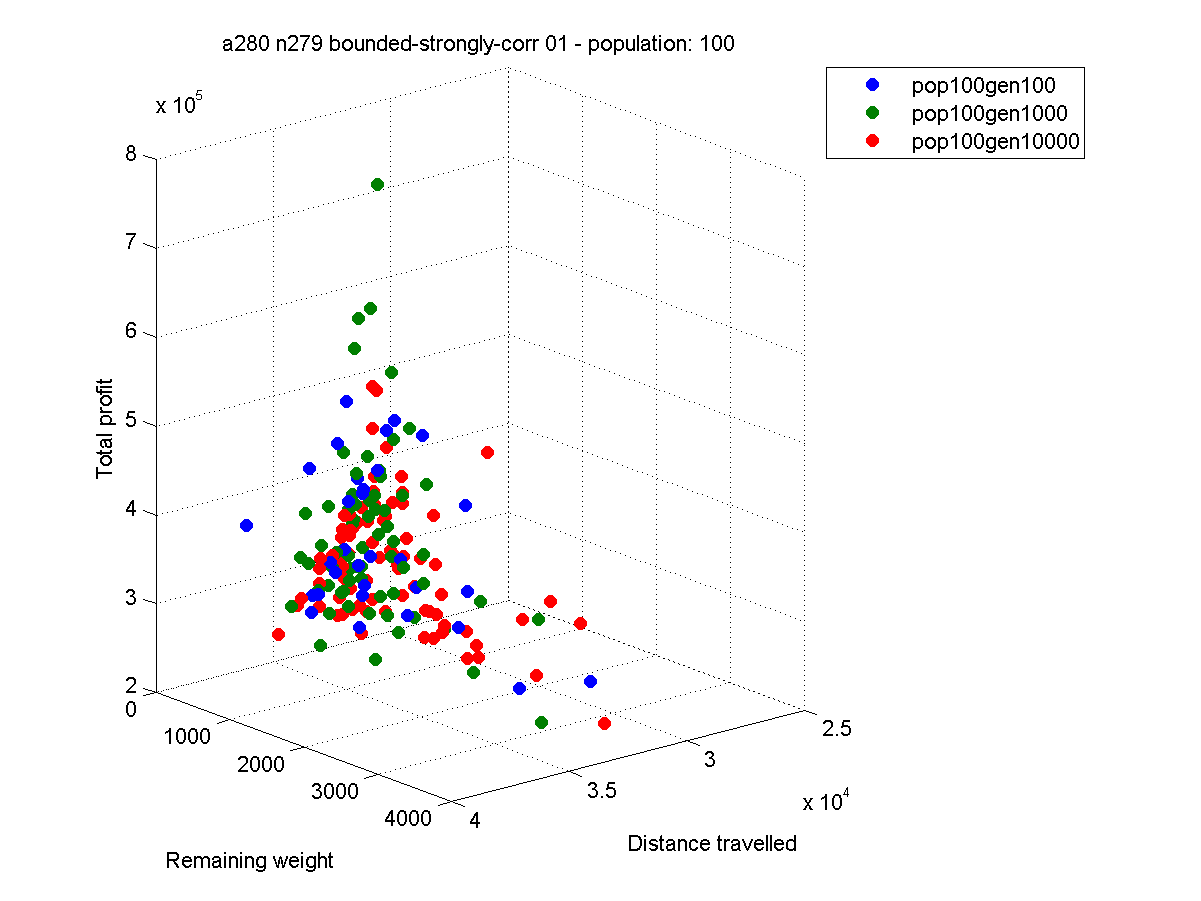
\includegraphics[width=.8\linewidth]{q4graphs/a280_n279_pop100.png}
  \label{fig:a280279100}
\end{minipage}
\end{figure}

\begin{figure}[h]
\centering
\begin{minipage}{.5\textwidth}
  \centering
  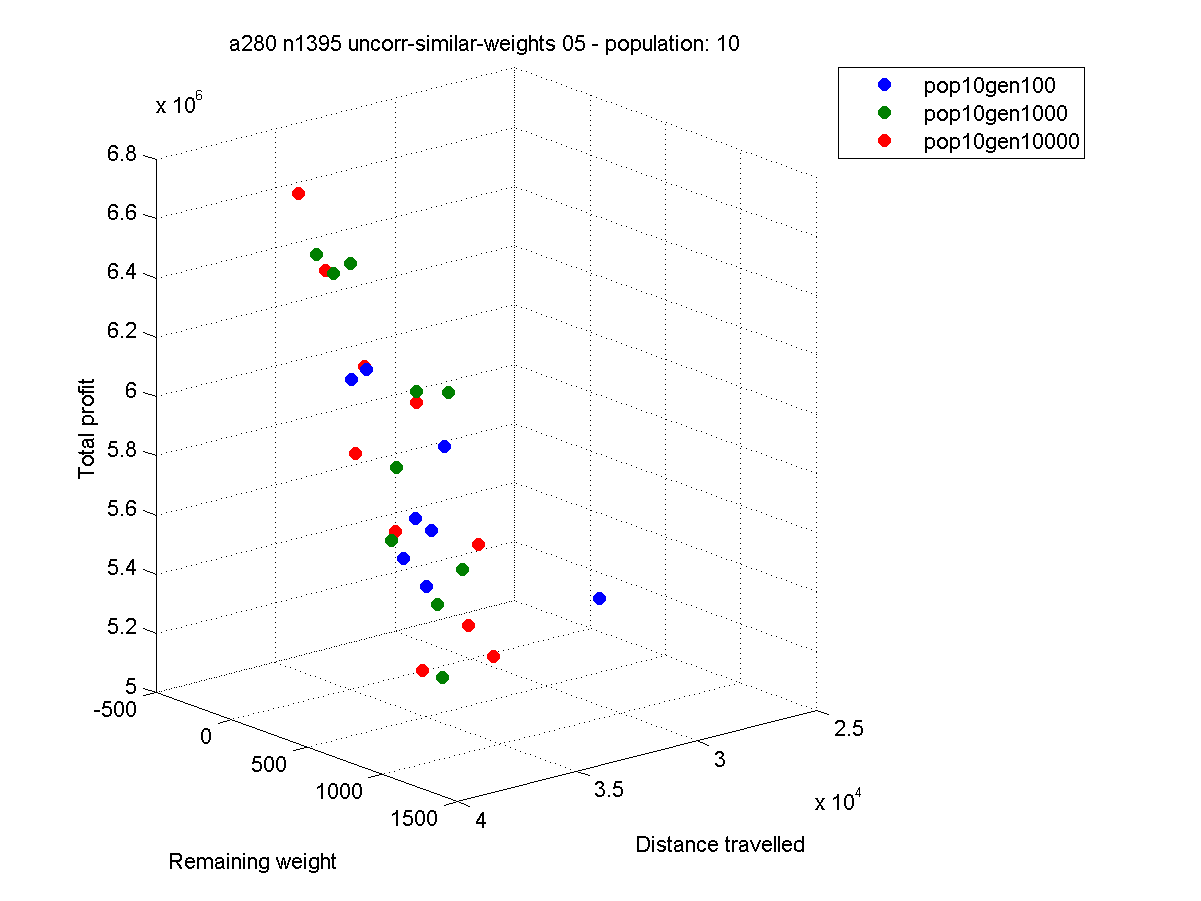
\includegraphics[width=.8\linewidth]{q4graphs/a280_n1395_pop10.png}
  \label{fig:a280139510}
\end{minipage}%
\begin{minipage}{.5\textwidth}
  \centering
  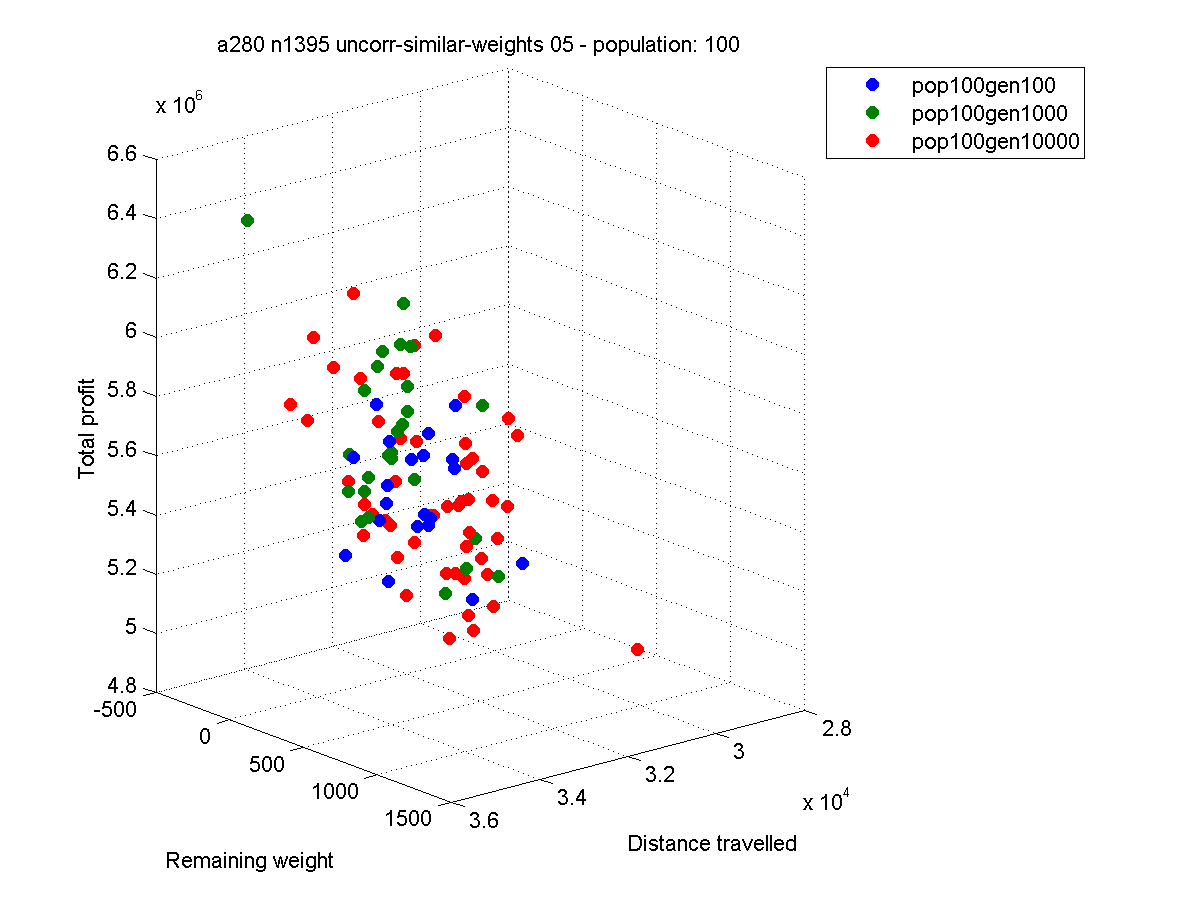
\includegraphics[width=.8\linewidth]{q4graphs/a280_n1395_pop100.png}
  \label{fig:a2801395100}
\end{minipage}
\end{figure}

\begin{figure}[h]
\centering
\begin{minipage}{.5\textwidth}
  \centering
  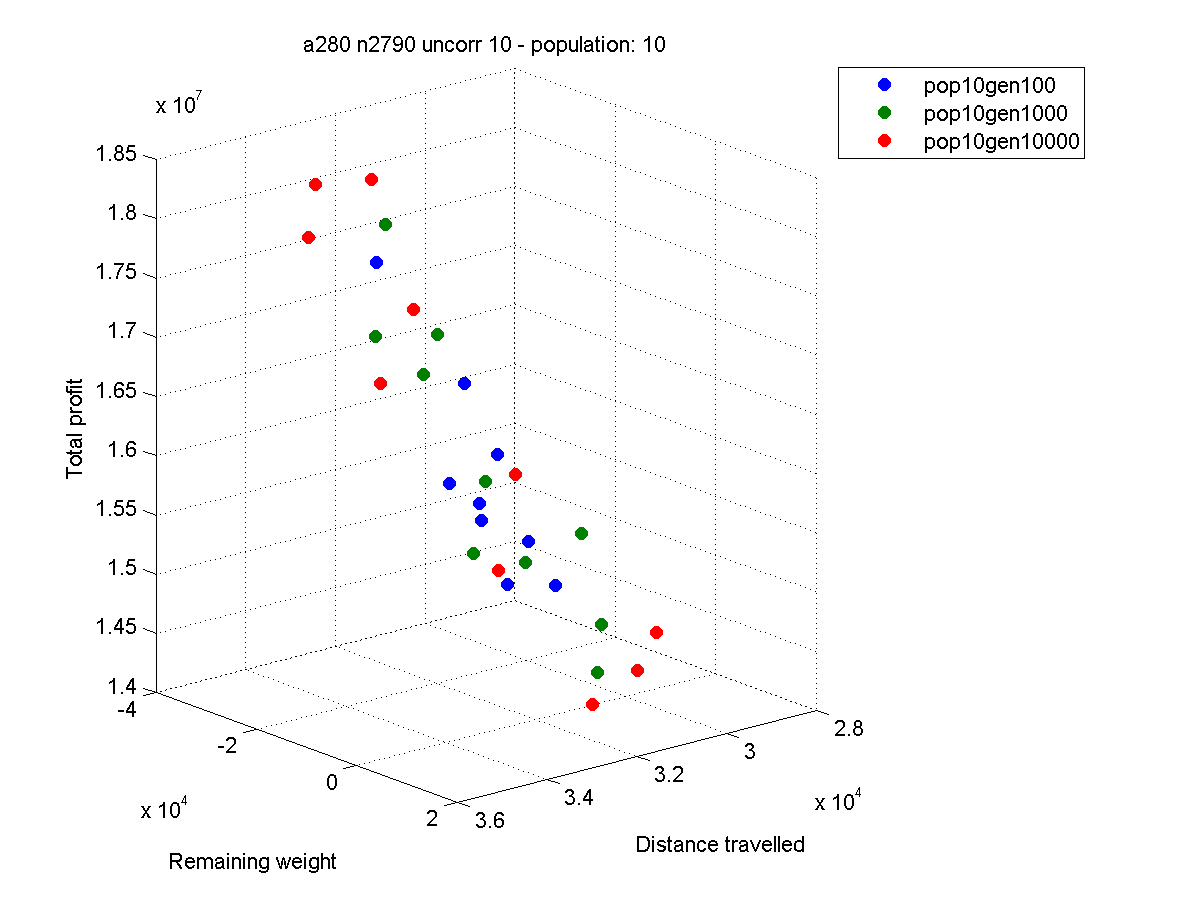
\includegraphics[width=.8\linewidth]{q4graphs/a280_n2790_pop10.png}
  \label{fig:a280279010}
\end{minipage}%
\begin{minipage}{.5\textwidth}
  \centering
  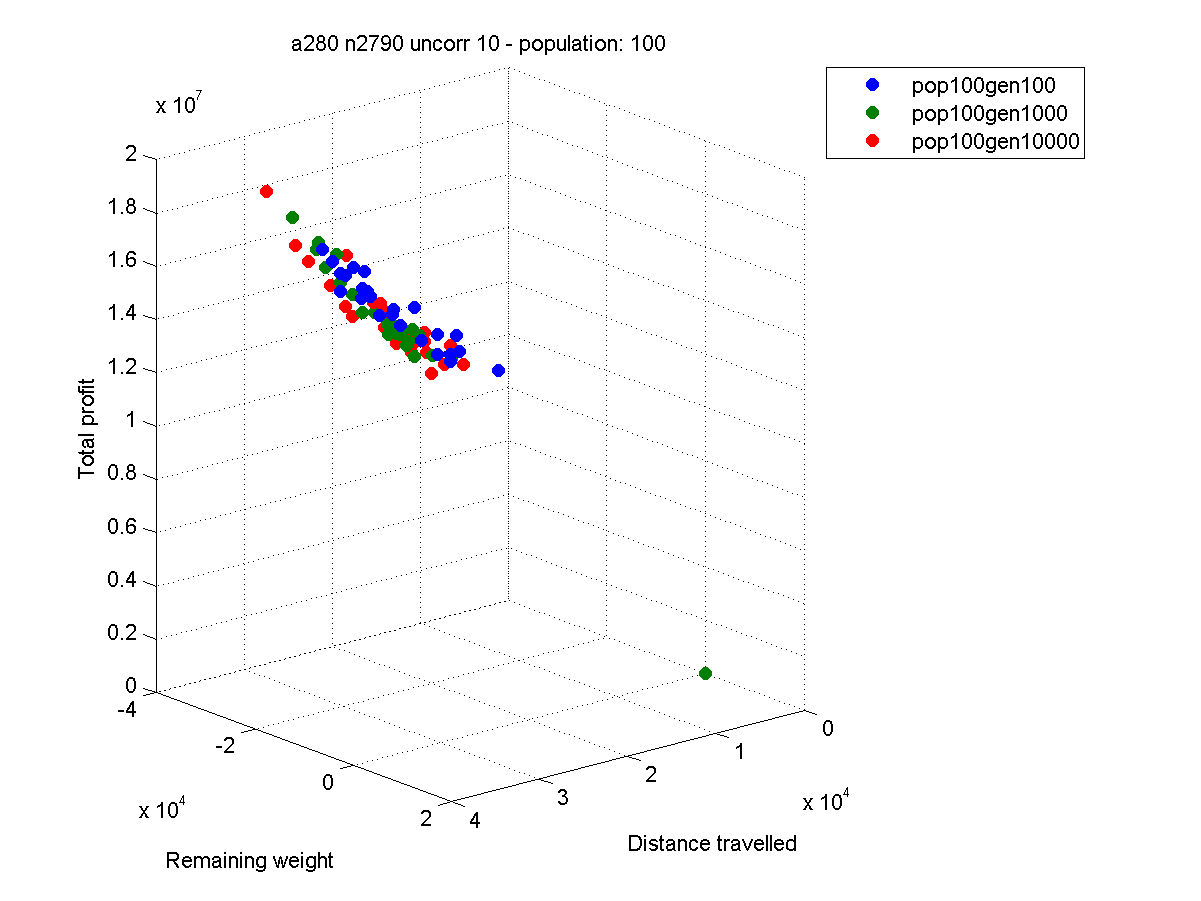
\includegraphics[width=.8\linewidth]{q4graphs/a280_n2790_pop100.png}
  \label{fig:a280279010}
\end{minipage}
\end{figure}

I don't understand why this last set of figures is randomly in the middle of the page but ok

latex y u do dis





\section*{Exercise 5}

Comparison of things and justification of things here

Visualisation of results here yo


\end{document}
